\section{System Models}
	This paper considers a robotic computation system consisting of a set of computation tasks and limited computation resources such as CPU cores. 
    The primary objective is to allocate resources effectively to optimize system performance in dynamic environments.
    This section introduces the system models, following notations from the real-time systems community~\cite{Buttazzo2011HardRC}.
    Frequently used notations are summarized in Table~\ref{notation_table}, while others are defined in context.
    % We use subscript to denote the \ith{i} instance of a vector. For example, $c_k$ denotes the \ith{k} element of vector $c$.

\begin{table}[]
\centering
\caption{Frequently-Used Notations}
\begin{tabular}{@{}ll@{}}
\toprule
Variables                                                             & Symbols         \\ \midrule
\ith{i} Computation task                                          & $\tau_i$        \\
Execution Time Distribution of $\tau_i$                                           & $\extDist{i}$           \\
Single Execution Time Value                                           & $c_i$           \\
Period                                                                & $T_i$           \\
Deadline                                                              & $D_i$           \\
Priority                                                              & $P_i$           \\
Priority Assignment Vector                                            & $\boldsymbol{P}$           \\
\begin{tabular}[c]{@{}l@{}}Response Time Probability Distribution of $\tau_i$  \end{tabular} & $\rtDist{i}$           \\
Scalar Response Time Value                                                         & $r_i$   \\
QoS budget list (candidate grid for $\tau_i$)                & $\boldsymbol{q-i}$     \\
QoS budget (selected option for $\tau_i$)                    & $q_i$     \\
Task's deadline miss threshold                                        & $\Theta_i$      \\
Task's importance                                                     & $w_i$           \\
Important task subset                                                  & $\boldsymbol{\tau}^{safe}$           \\
Environment-dependent task (env-dependent $\extDist{i}$)                & $\tau^E_i$      \\
QoS-configurable task (carries a QoS budget list $\boldsymbol{q-i}$)            & $\tau^Q_i$      \\
Higher-priority task set of $\tau_i$ (given $\boldsymbol{\tau},\boldsymbol{P},\boldsymbol{Q}$) & $\text{hp}(i;\boldsymbol{\tau},\boldsymbol{P},\boldsymbol{Q})$ \\  \midrule
\begin{tabular}[c]{@{}l@{}}Environment vector at the\\ $k$-th interval ($k$: interval index)\end{tabular}         & $\textbf{E}_k$           \\
$\tau_i$'s execution time distribution prediction function & $\mathcal{F}_i(\textbf{E}) \rightarrow \extDist{i} $ \\
Safety-Performance metric                                                             & $\textbf{SP}$   \\
$s$-th challenger solution during search                              & $\boldsymbol{P}^{(s)},\boldsymbol{Q}^{(s)}$ \\
Champion solution while evaluating the $s$-th challenger              & $\boldsymbol{P}^{(s)*},\boldsymbol{Q}^{(s)*}$ \\
Performance Metric                                                    & $\mathcal{P}()$ \\
Safety Metric                                                         & $\mathcal{S}()$ \\
Probability of an event                                                    & $\text{Pr}(event)$ \\
Probability Distribution & $\mathcal{D}$ \\
\\\bottomrule
\end{tabular}
\label{notation_table}
\end{table}
	
	
	\subsection{Computation Tasks}
    \label{section: system_model_tasks}
    A computation task represents an independent high-level application, such as motion planning or obstacle detection.
    For simplicity of presentation, we assume each task uses one CPU core each time.
    How to optimize other types of tasks models is discussed in Section~\ref{section: gang}.

	
	Most robotic tasks are modeled as periodic tasks\footnote{Tasks with non-constant periods, called sporadic tasks, have a minimum arrival interval between successive executions. These sporadic tasks are often treated as periodic tasks during schedulability analysis to simplify the modeling process} $\tau$. 
    We use $\boldsymbol{\tau}$ to denote the task set under consideration, $\tau_i$ to denote the \ith{i} task.
    Each task $\tau_i$ is characterized by five parameters: probability distribution of execution time $\extDist{i}$, period $T_i$, deadline $D_i$, and its Quality-of-Service (QoS) budget $q_i$:
	\begin{equation}
		\tau_i: [\extDist{i}, T_i, D_i, q_i]
		\label{eq_notation_task}
	\end{equation}
	

	\begin{definition}[Period, $T_i$]
		A task $\tau_i$ releases one job\footnote{According to Buttazzo~\cite{Buttazzo2011HardRC}, ``Periodic tasks consist of an infinite sequence of identical activities, called instances or \textit{jobs}, that are regularly activated at a constant rate.''} $J$ for execution every $T_i$ time units.
	\end{definition}
    In other words, the periodic task $\tau_i$ needs to be run for one time every $T_i$ time units.
	
	\begin{definition}[Deadline, $D_i$]
		Deadline $D_i$ refers to the maximum amount of time that a job must be completed to avoid causing potential damage to the system.
	\end{definition}
	
	

	% The deadline definition above is the same as the \textit{relative deadline} used in the real-time system community. 
    In most cases, the deadline $D_i$ is no larger than the period $T_i$~\cite{Buttazzo2011HardRC, Wang2023RTAS}. 
	In experiments, we use the implicit deadline configurations for simplicity: $D_i = T_i$.
	However, the propsoed system also works well for systems with other deadlien configurations.


	\begin{definition}[Execution time, $\extDist{i}$]
		A task's execution time is a probability distribution of the time needed by one standard processor\footnote{Different processors may have different speed. 
		A standard processor in this context means that the execution time is measured on a processor whose speed is normalized.} to finish its execution without interruption.
	\end{definition}

    The task's execution time is modeled as a probability distribution~\cite{Maxim2013ResponseTA}, reflecting variability due to factors like input data, operating system (OS) behavior, and hardware performance.
    This approach captures uncertainty while avoiding pessimistic worst-case assumptions.
    In experiments, due to the stringent need to maintain low scheduling overhead, we assume the execution time follows Gaussian distribution to reduce the optimization cost. 
	This assumption is a safe assumption as long as the gaussian distribution is a safe upper-bound of the true underlying execution time distribution.
	
	For example, motion planning may adopt a searching-based anytime algorithm, which takes the running-time limit as its QoS budget: a larger budget lets the search find a higher-quality plan (and runs longer).
	
	Depending on whether tasks' execution time distribution is controlled by external environments, or the internal scheduling algorithms, we can categorize tasks into:
	\begin{itemize}
	\item environment-dependent tasks
	\item QoS-configurable tasks
	\end{itemize}
	\begin{definition}[QoS budget, $q_i$]
		\label{def_task_config}
		A task $\tau_i$'s Quality-of-Service (QoS) budget $q_i$ is the parameter that influences the task's execution time distribution and output quality.
		For anytime algorithms, the QoS budget is the maximum execution-time limit allocated to the algorithm: a larger budget yields a higher-quality output (and a longer execution time).
	\end{definition}
	Only anytime algorithms have a QoS budgets. Tasks where each invocation terminates on its own independent of computation budgets do not have a QoS budget and therefore do not involve QoS optimization.
	
	In this paper, we focus on the running-time limit as the QoS budget because it governs both the performance and safety of a task.
	Other parameters can be incorporated into our framework in a similar way.

	Building on these notions, we introduce symbols for two task types referenced throughout the paper.
	An \emph{environment-dependent task}, denoted $\tau^E_i$, is a task whose execution-time distribution $\extDist{i}$ varies with the environment vector $\textbf{E}$ (Section~\ref{section_et_model}); a \emph{QoS-configurable task}, denoted $\tau^Q_i$, is a task that carries a QoS budget $q_i$ (Definition~\ref{def_task_config}).
	Tasks that are neither are referred to as \emph{normal tasks}.
	Section~\ref{section: simulation} details how task sets of these types are generated for our experiments.
	
	
\begin{figure*}[htbp]
\centering
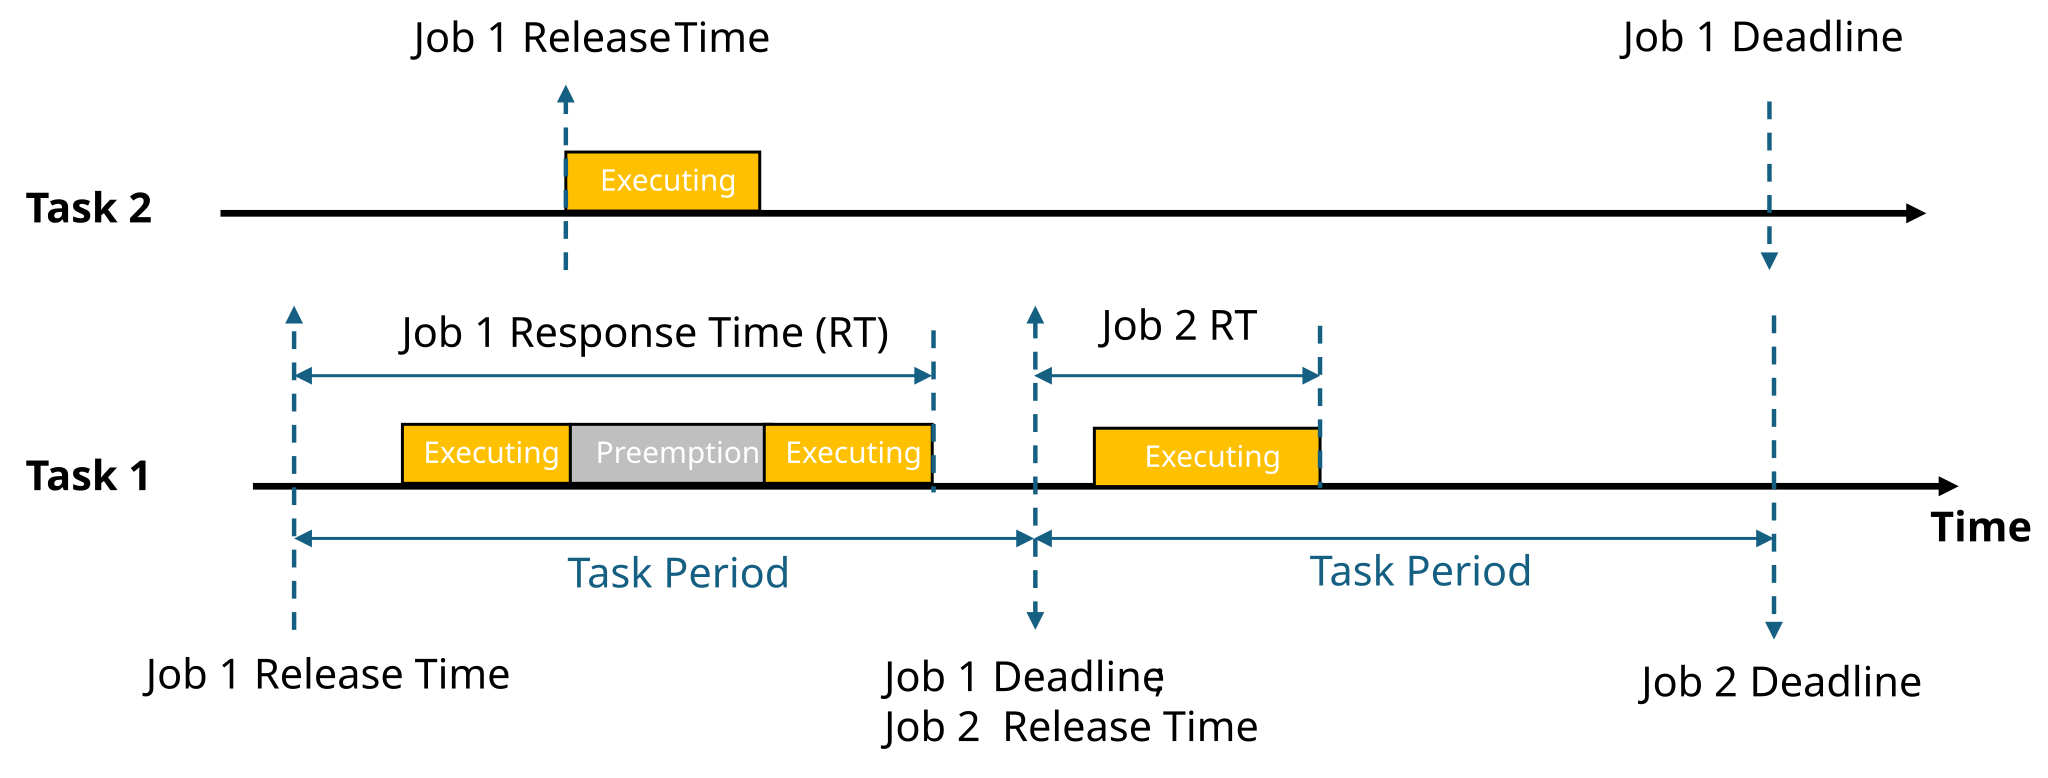
\includegraphics[width=0.8\textwidth]{pictures/RTS_concepts.pdf}
\caption{Concepts adopted from the Real-Time Systems Area. The figure above shows two tasks' scheduling, where task 2 has higher priority than task 1 and both are scheduled to run on the same CPU core. When task 2 releases a job to execute, it preempts task 1's job. The job 1 of task 1 continues execution after task 2's job 1 finishes execution.
}
\label{fig_rts_concepts}
\end{figure*}
    
	
	\subsection{Computation Platform}
	\label{section_rta_distribution}
    This paper uses a widely-adopted computation platform configurations~\cite{Ash23RAL, Wang2023OptimizingLET, Verucchi2020LatencyAwareGO}.
	The computation platform is modelled as a multi-core system where each task is assigned to a known core using partitioned scheduling~\cite{Buttazzo2011HardRC}.
	The system disables task migration to reduce scheduling overheads and provides more predictable response time~\cite{Brandenburg2016GlobalSN}.
    Each task is assigned a unique priority $P_i$, which could change from time to time based on scheduling algorithms.
    Under preemptive scheduling, higher-priority tasks could preempt lower-priority tasks when high-priority tasks become ready, which are paused and resumed later.
    In this paper, we focus on soft real-time systems, where tasks that miss deadlines by small margins can still contribute to system functionality.
	
	We use priority assignments to describe the relative importance of tasks:
	\begin{definition}[Priority Assignments, $\boldsymbol{P}$]
		A priority assignment vector $\boldsymbol{P}$ for a task set $\boldsymbol{\tau}$ is a complete ordered sequence of tasks $\boldsymbol{\tau}$, where higher-priority tasks appear earlier.
	\end{definition}
    
    In most operating systems such as Linux, the priority assignment needs to be converted into priority values to be useful, see more in Section~\ref{section_pa_values}.
	
	\subsection{Schedulability Analysis}
	\label{sectino_schedulability_analysis}

    \textit{Schedulability} determines whether all tasks can meet their deadline requirements under a given scheduling algorithm.
    There are two types of schedulability: \textit{Hard} Schedulability, where all tasks must always finish before their deadlines;
    \textit{Soft} Schedulability, where the probability of any task missing its deadline is below a given threshold (some papers may use a slightly different definition).
    
	This paper focuses on soft schedulability because it is not only more general than hard schedulability, but also more practical for robotic systems and balances resource constraints with system performance.
    
	
	Response time analysis (RTA) is one of the most well-studied methods to analyze schedulability:
	\begin{definition}[Response time $r_i$]
		A task $\tau_i$'s response time $r_i$ includes its execution time $c_i$ and the time that it waits to obtain the required computation resources (\eg being preempted).
	\end{definition}
	Considering the random nature of execution, using a probability distribution rather than a single worst-case value to quantify the response time is more accurate and less pessimistic:
	\begin{definition}[Response time distribution $\rtDist{i}$]
		A task $\tau_i$'s response time distribution $\rtDist{i} = \{r_i^{(k)}: p_i^{(k)}\}$ is a discrete probability distribution of $k$ items, where each item describes that the probability of having response time as $r_i^{(k)}$ is $p_i^{(k)}$.
	\end{definition}
    
	Response time distribution can be obtained either experimentally or analytically. 
	The analytical methods are much faster and simpler than the experimental methods but are also more pessimistic. 
	Check Section~\ref{section_rta} for more details.
	
	